% Options for packages loaded elsewhere
\PassOptionsToPackage{unicode}{hyperref}
\PassOptionsToPackage{hyphens}{url}
%
\documentclass[
]{article}
\usepackage{amsmath,amssymb}
\usepackage{iftex}
\ifPDFTeX
  \usepackage[T1]{fontenc}
  \usepackage[utf8]{inputenc}
  \usepackage{textcomp} % provide euro and other symbols
\else % if luatex or xetex
  \usepackage{unicode-math} % this also loads fontspec
  \defaultfontfeatures{Scale=MatchLowercase}
  \defaultfontfeatures[\rmfamily]{Ligatures=TeX,Scale=1}
\fi
\usepackage{lmodern}
\ifPDFTeX\else
  % xetex/luatex font selection
\fi
% Use upquote if available, for straight quotes in verbatim environments
\IfFileExists{upquote.sty}{\usepackage{upquote}}{}
\IfFileExists{microtype.sty}{% use microtype if available
  \usepackage[]{microtype}
  \UseMicrotypeSet[protrusion]{basicmath} % disable protrusion for tt fonts
}{}
\makeatletter
\@ifundefined{KOMAClassName}{% if non-KOMA class
  \IfFileExists{parskip.sty}{%
    \usepackage{parskip}
  }{% else
    \setlength{\parindent}{0pt}
    \setlength{\parskip}{6pt plus 2pt minus 1pt}}
}{% if KOMA class
  \KOMAoptions{parskip=half}}
\makeatother
\usepackage{xcolor}
\usepackage[margin=1in]{geometry}
\usepackage{longtable,booktabs,array}
\usepackage{calc} % for calculating minipage widths
% Correct order of tables after \paragraph or \subparagraph
\usepackage{etoolbox}
\makeatletter
\patchcmd\longtable{\par}{\if@noskipsec\mbox{}\fi\par}{}{}
\makeatother
% Allow footnotes in longtable head/foot
\IfFileExists{footnotehyper.sty}{\usepackage{footnotehyper}}{\usepackage{footnote}}
\makesavenoteenv{longtable}
\usepackage{graphicx}
\makeatletter
\def\maxwidth{\ifdim\Gin@nat@width>\linewidth\linewidth\else\Gin@nat@width\fi}
\def\maxheight{\ifdim\Gin@nat@height>\textheight\textheight\else\Gin@nat@height\fi}
\makeatother
% Scale images if necessary, so that they will not overflow the page
% margins by default, and it is still possible to overwrite the defaults
% using explicit options in \includegraphics[width, height, ...]{}
\setkeys{Gin}{width=\maxwidth,height=\maxheight,keepaspectratio}
% Set default figure placement to htbp
\makeatletter
\def\fps@figure{htbp}
\makeatother
\setlength{\emergencystretch}{3em} % prevent overfull lines
\providecommand{\tightlist}{%
  \setlength{\itemsep}{0pt}\setlength{\parskip}{0pt}}
\setcounter{secnumdepth}{5}
% definitions for citeproc citations
\NewDocumentCommand\citeproctext{}{}
\NewDocumentCommand\citeproc{mm}{%
  \begingroup\def\citeproctext{#2}\cite{#1}\endgroup}
\makeatletter
 % allow citations to break across lines
 \let\@cite@ofmt\@firstofone
 % avoid brackets around text for \cite:
 \def\@biblabel#1{}
 \def\@cite#1#2{{#1\if@tempswa , #2\fi}}
\makeatother
\newlength{\cslhangindent}
\setlength{\cslhangindent}{1.5em}
\newlength{\csllabelwidth}
\setlength{\csllabelwidth}{3em}
\newenvironment{CSLReferences}[2] % #1 hanging-indent, #2 entry-spacing
 {\begin{list}{}{%
  \setlength{\itemindent}{0pt}
  \setlength{\leftmargin}{0pt}
  \setlength{\parsep}{0pt}
  % turn on hanging indent if param 1 is 1
  \ifodd #1
   \setlength{\leftmargin}{\cslhangindent}
   \setlength{\itemindent}{-1\cslhangindent}
  \fi
  % set entry spacing
  \setlength{\itemsep}{#2\baselineskip}}}
 {\end{list}}
\usepackage{calc}
\newcommand{\CSLBlock}[1]{\hfill\break\parbox[t]{\linewidth}{\strut\ignorespaces#1\strut}}
\newcommand{\CSLLeftMargin}[1]{\parbox[t]{\csllabelwidth}{\strut#1\strut}}
\newcommand{\CSLRightInline}[1]{\parbox[t]{\linewidth - \csllabelwidth}{\strut#1\strut}}
\newcommand{\CSLIndent}[1]{\hspace{\cslhangindent}#1}
\usepackage{lscape}
\usepackage{booktabs}
\usepackage{longtable}
\usepackage{array}
\usepackage{multirow}
\usepackage{wrapfig}
\usepackage{float}
\usepackage{colortbl}
\usepackage{pdflscape}
\usepackage{tabu}
\usepackage{threeparttable}
\usepackage{threeparttablex}
\usepackage[normalem]{ulem}
\usepackage{makecell}
\usepackage{xcolor}
\ifLuaTeX
  \usepackage{selnolig}  % disable illegal ligatures
\fi
\usepackage{bookmark}
\IfFileExists{xurl.sty}{\usepackage{xurl}}{} % add URL line breaks if available
\urlstyle{same}
\hypersetup{
  pdftitle={When Forgiveness Backfires: Rejection Sensitivity and Cooperative Behavior Following Exposure to Adaptive Forgiving Agents},
  pdfauthor={Ismail Guennouni1*, Georgia Koppe2, Christoph Korn3},
  hidelinks,
  pdfcreator={LaTeX via pandoc}}

\title{When Forgiveness Backfires: Rejection Sensitivity and Cooperative Behavior Following Exposure to Adaptive Forgiving Agents}
\author{Ismail Guennouni\textsuperscript{1}*, Georgia Koppe\textsuperscript{2}, Christoph Korn\textsuperscript{3}}
\date{}

\begin{document}
\maketitle
\begin{abstract}
Can exposure to forgiving behavior improve cooperative outcomes, and does Rejection Sensitivity (RS) moderate this effect? This randomized controlled experiment explores these questions using a novel approach with Hidden Markov Model (HMM)-based artificial agents in repeated trust games (RTGs). Participants (N = 206), pre-screened for high or low RS, interacted with either consistently behaving or more forgiving co-players, which were in reality HMM agents. Unexpectedly, exposure to forgiving agents led to reduced cooperation in subsequent interactions. Control group participants maintained consistent behavior. RS levels influenced perceptions of the agent's cooperativeness but did not significantly affect behavioral outcomes, revealing a perception-behavior dissociation. These findings challenge assumptions about fostering cooperation through simple exposure to positive interactions and highlight the importance of accounting for negative contrast effects when designing such interventions. They also demonstrate the potential of HMM-based artificial agents for studying interactive social dynamics, offering a methodological advancement for future research. Our results suggest the need for nuanced interventions that gradually shape expectations and behaviors to foster cooperative outcomes, particularly for individuals with high rejection sensitivity.
\end{abstract}

\small

\textsuperscript{1} \emph{Central Institute of Mental Health, Medical Faculty Mannheim/Heidelberg University, Germany}

\textsuperscript{2} \emph{Faculty of Mathematics and Computer Science, Heidelberg University, Germany}

\textsuperscript{3} \emph{Department of General Psychiatry, Section Social Neuroscience, Heidelberg University, Germany}

\textsuperscript{*} \emph{Corresponding author. Address: Central institute of Mental Health, J5, Mannheim, Germany. Email: \href{mailto:ismail.guennouni@zi-mannheim.de}{\nolinkurl{ismail.guennouni@zi-mannheim.de}}}

\vspace{1cm}

\textbf{Keywords} : Social Trust; Forgiveness Intervention; Rejection Sensitivity; Interpersonal Dynamics; Hidden Markov Models

\vspace{1cm}

\textbf{Highlights:}

\begin{itemize}
\item
  Exposure to forgiving artificial agents unexpectedly led to reduced cooperation in subsequent interactions, challenging assumptions about fostering trust through positive experiences
\item
  Rejection sensitivity influenced perceptions of artificial agents' cooperativeness but not behavioral outcomes, revealing a dissociation between perception and behavior
\item
  Novel Hidden Markov Model-based artificial agents provide adaptive, human-like behavior in trust games, allowing for precise control of ``cooperative'' and ``forgiving'' strategies while maintaining experimental control of co-player strategies
\end{itemize}

\pagebreak

\section{Introduction}\label{introduction}

Trust is fundamental to human social interactions, facilitating seamless relations at both interpersonal and intergroup levels. The study of psychopathology has linked deficits in trust-based constructs to the development of mental health disorders (Fonagy and Campbell 2017). Individuals with personality disorders (PD) often struggle to form and maintain social connections, a difficulty reflected in uncooperative behaviors -- a marker for the severity of PD symptoms (Herpertz and Bertsch 2014; Mulder et al. 1999).

One explanation for such social challenges lies in early caregiver experiences. Attachment theory (Bowlby 1978) suggests that the quality of these relationships shapes our capacity for secure attachments and trust. Individuals with higher levels of insecure attachment may recall negative trust-related experiences more easily, report fewer positive trust experiences, and use less constructive coping strategies when trust is broken (Mikulincer 1998). These insecure attachment patterns are often associated with heightened rejection sensitivity (RS), a tendency to anxiously expect, readily perceive, and intensely react to rejection (Downey and Feldman 1996; Downey, Khouri, and Feldman 1997). RS has been linked to the development of various mental health conditions, including depression, anxiety, personality disorders, and self-harm (Gao et al. 2017). A recent meta-analysis revealed prosocial behavior and interpersonal trust as two key processes of interpersonal functioning that are markedly impaired in PDs and which are likely to contribute to interpersonal dysfunction in this population (Hepp and Niedtfeld 2022). The interaction of rejection sensitivity and trust-based constructs has been explored, particularly in Borderline Personality Disorder (BPD). Miano et al. (2013) and Richetin et al. (2018) found that rejection sensitivity mediated the relationship between BPD features and lower trust appraisal. Abramov et al. (2022) found that higher baseline feelings of rejection in individuals with BPD predict slower trust formation and less pronounced declines in trust following trust violations during the trust game. However, the interaction between trustworthiness and rejection sensitivity hasn't been studied as extensively in other personality disorders or in non-clinical populations, leaving a gap in our understanding of how these constructs might interplay. Could an ingrained sensitivity to rejection contribute to reduced pro-social behavior such as a failure to show trustworthiness?

If indeed RS contributes to interpersonal dysfunction through failure to show trustworthiness, could exposing those who exhibit it to cooperative and forgiving interaction partners lead to improved interpersonal outcomes? Research in the fields of behavioral economics and psychology has explored how positive social interactions influence cooperation and pro-social behavior. The use of the repeated trust game (RTG), a well-established experimental approach, has allowed for the analysis of the development of trust through ongoing interactions (Joyce, Dickhaut, and McCabe 1995). In this paradigm, cycles of mutual trust, where each party's trust is reciprocated with trustworthiness, have the effect of enhancing cooperative behaviors even among individuals who are initially inclined to be distrustful (King-Casas et al. 2005). Fowler and Christakis (2010) studied behavior in social networks interacting in a public goods game and found that cooperative behavior tends to cluster, suggesting that exposure to cooperative peers can lead to more cooperative behavior. Similarly, research on social learning theory (Bandura 1977) has long demonstrated that individuals learn and model the behavior of those around them, indicating that if someone is consistently exposed to cooperative and positive individuals, they're likely to emulate this behavior. These insights highlight that engaging with compassionate and forgiving others can be an effective method for mitigating deeply ingrained mistrust and potentially fostering trustworthy behavior.

In this study, we use a randomized controlled online experiment to test whether exposing participants with varying RS levels to forgiving and more cooperative co-players results in more trustworthy behavior and a repair of potential breakdowns in RTG cooperation. To simulate realistic social interaction while maintaining a high degree of experimental control, we take a novel paradigmatic approach: We use generative models of how humans play the RTG to design an agent that plays the role of the investor, based on Hidden Markov Models (HMMs) fitted to real players' data. A key aspect of these agents is that their actions depend on a latent ``trust state'' which reacts dynamically to the trustees' returns, simulating real-life trust-building scenarios. An advantage of having such a generative model of behavior is the possibility of controlling different aspects of the agent's strategy such as its general policy, the propensity to cooperate actively, or the propensity to retaliate after breakdowns of cooperation.

We pre-screened participants for high or low rejection sensitivity (RS) using a validated questionnaire, then assigned them exclusively to the trustee role in a series of trust games. After playing a 15-round RTG with a human-like HMM investor, they were randomly assigned to either a Control or Manipulation condition. In the Manipulation condition, participants were exposed over three RTGs to HMM investors designed with a limited propensity for retaliation, potentially mitigating ingrained mistrust. In the Control condition, participants played three RTGs against the same human-like HMM. After this exposure phase, all participants played another 15-round RTG with a human-like HMM investor. We expect those exhibiting high RS to be more responsive to the pre-programmed change in the agent's cooperativeness and retaliation propensity. We also hypothesize that those in the Manipulation condition would behave more cooperatively and have a lower propensity to retaliate to the co-player's defection after the exposure phase, with those in the higher RS group showing a bigger effect.

\section{Methods}\label{methods}

\subsection{Participants}\label{participants}

To have participants with large differences in RS, a total of 1195 participants were pre-screened on the Prolific Academic platform (prolific.co) using the Rejection Sensitivity Questionnaire (RSQ) to finally select two similarly sized groups: One with high RS (RSQ score \textgreater{} 15) and the other with low RS (RSQ score \textless{} 10) totalling 206 participants (56\% female). These were then invited through prolific to take part in the main experiment study. The required sample size was determined using an a priori power analysis to have an 80\% probability to detect a small effect size with a 5\% type I error rate in a repeated measures ANOVA with between factors. The mean age of participants was 34.6 years, with an 11.9 years standard deviation. Participants were paid a fixed fee of £6 plus a bonus payment dependent on their performance that averaged £0.5.

\subsection{Design and Procedure}\label{design-and-procedure}

The experiment had a 2 (Condition: Manipulation or Control) by 2 (RS : High or Low) by 2 (Game: Trust-Game Pre Manipulation, Trust-Game Post Manipulation) design, with repeated measures on the third factor (Figure \ref{fig:HMMPanels}.A). Participants within each pre-screened group were randomly assigned to one of the two levels of the Condition factor. The games were designed and implemented online using Empirica v1 (Almaatouq et al. 2021). The planned experiment received approval from the University of Heidelberg's Medical Faculty ethics commission (ID:S-708/2023) and the experiment was performed in accordance with the ethics board guidelines and regulations. All participants provided informed consent prior to their participation.

\subsection{Tasks and Measures}\label{tasks-and-measures}

\subsubsection{Repeated Trust Game}\label{repeated-trust-game}

Participants played a 15-round RTG (Joyce, Dickhaut, and McCabe 1995) in the trustee role against a computer-programmed investor. On each round the investor is endowed with 20 units and decides how much of that endowment to invest. This investment is tripled and the trustee then decides how to split this tripled amount between them and the investor. If the trustee returns more than one third of the amount, the investor makes a gain. Each player was represented with an icon with the participant always on the left of the screen and the co-player on the right. The participants were able to choose the icon that represents them at the start of the experiment. The icon representing the co-player changed at the start of each new game, to simulate a new interaction partner. Participants were not told they were facing computerised co-players. We chose to simulate the behavior of a human interaction partner through allowing for a delay whilst pairing with new opponents as the start of each game as well as programming the agents to respond during each round after a varying time lapse (randomly chosen between 5 and 10 seconds).

The computerised investor consisted of a hidden Markov model (HMM) trained on an independent existing behavioral RTG data set of human investors. This data-driven approach thus sought to learn an investor strategy that mimics human-like interactions. The data set used for training consists of 388 ten round games with the same player (full details can be found in the Supplementary Information). On this data set, the HMM was inferred with three latent states that could be interpreted as reflecting a ``low-trust'', a ``medium-trust'', and a ``high-trust'' state. A separate output distribution, that maps each HMM state onto possible investments from 0 to 20 separately, is learned (Figure \ref{fig:HMMPanels}.B). In analogy to the latent states, these distributions can be interpreted as reflecting ``low-trust'', ``medium-trust'', or ``high-trust'' dispositions. Finally, the HMM is specified by transition probabilities that describe the transition between states. The probability of these transitions was modelled as a function of their net return (i.e return - investment) in the previous round (see Figure \ref{fig:HMMPanels}.C)). The initial state for the HMM investor in each instance of the game was set to the ``mid-trust'' state. Details on how the HMM state conditional probabilities and transition functions are specified can be found in the supplement.

In order to instigate a potential breakdown of trust, thereby allowing us to probe efforts to repair it, the computerised agent was programmed to provide a low investment on round 12 (pre-manipulation) and round 13 (post-manipulation). On all other rounds, the investor's actions were determined by randomly drawing an investment from the state-conditional distribution, with the state over rounds determined by randomly drawing the next state from the state-transition distribution as determined from the net return on the previous round (disregarding the net return immediately after the pre-programmed low investment rounds).

\subsection{Manipulation}\label{manipulation}

In all phases of the RTG other than the `Exposure phase' (Figure \ref{fig:HMMPanels}.A), participants interacted with this human-like HMM. In the `Manipulation' Condition of the exposure phase, however, the parameters of this HMM were adjusted to design a `forgiving' and ultimately more cooperative agent. To achieve this, we changed the state transition probabilities of the HMM such that it becomes impossible for it to remain in a low trust state, effectively setting the transition probability for remaining in a ``low-trust'' state to 0. The resulting transition function is shown in Figure \ref{fig:HMMPanels}.D. The policies conditional on the latent states and the transition function in the other latent states remain unchanged.

\begin{landscape}
\begin{figure}

{\centering 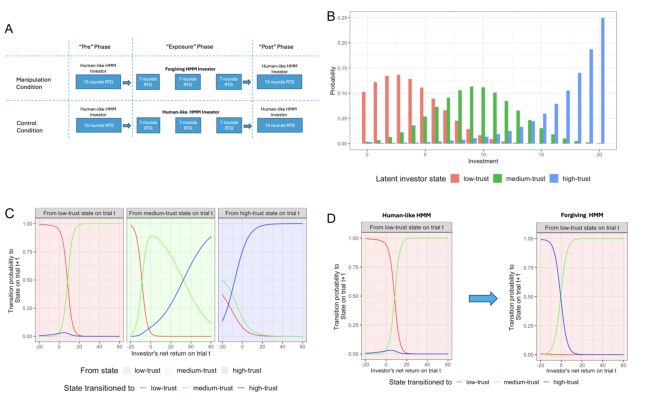
\includegraphics[width=1\linewidth,height=1\textheight]{article_files/figure-latex/HMMPanels-1} 

}

\caption{\small{A: A timeline of the experiment for both conditions. The RTG is played in dyads, with participants always assigned the role of the trustee and the HMM agent that of the investor. The investor is endowed with 20 units at the start of each round. They need to decide how much of that endowment they want to invest with the trustee. The investment is then multiplied by a factor of 3 and sent to the trustee who needs to decide how much of the multiplied investment they want to send back to the investor. The difference between conditions is the type of agents participants are exposed to in the exposure phase. Panels B - D: We construct the artificial investor agent by fitting a three-state hidden Markov model to data of human investors engaged in the 10 round RTG against human trustees. From the fitted HMM, we get the distribution of investments by the human-like agent, conditional on its latent state as shown in Panel B. The fitted HMM also yields the transition probability of the agent to a state on trial t+1 as a function of the net return (difference between the investment sent and the amount received in return) on trial t as shown in Panel C. Each plot in Panel C represents a different starting latent state on trial t, and each line represents the probability of transitioning to a particular state in trial t+1. Panel D shows the transition probabilities of the forgiving HMM agent in the low trust state. Unlike the human-like HMM, the forgiving HMM always transitions out of the low-trust state, and is more likely to end up in a high-trust state, as a proxy for coaxing behavior. Transitions in the medium and high trust states were identical for both agents.}}\label{fig:HMMPanels}
\end{figure}
\end{landscape}

\subsection{Procedure}\label{procedure}

At the start of the experiment, participants provided informed consent and were instructed the study would consist of three phases in which they would face a different other player. Participants were told their goal was to maximise the number of points in all phases. They were not told the number of rounds of each phase. Participants were randomly assigned to either a Control or Manipulation condition. The timeline of the experiment is shown in Figure \ref{fig:HMMPanels}.A. Phase one (``pre'') consisted of a 15 round RTG in which participants took the role of trustee, facing the same investor over all 15 rounds. On each round, after being informed about the amount sent by the investor participants decided how much of the tripled investment to return to the investor, before continuing to the next round. Phase 2 (``exposure'') consisted of three 7-round RTGs. Participants in the Manipulation condition faced the forgiving HMM investor and rated the agent on the same attributes as in the pre-manipulation phase. Those in the Control condition faced the same human-like HMM agent as in the ``pre'' phase and rated each co-player on the same attributes. To keep the experience similar to the ``pre'' phase, the agent in the Control condition was also designed to send a very low investment in round 5 of each of the three games. In the post-manipulation phase (``post''), participants in both conditions faced the same human-like HMM as in ``pre'' phase.

At the beginning of each game in all three phases, participants were told they would face a new player and had to wait to be paired with an available co-player. This simulated the waiting time in real social interaction tasks. After completing each RTG in each phase, participants rated how cooperative and forgiving they perceived the co-playerr to be, and whether they would like to play with them again (all on a scale from 1 to 10 with 10 being the most positive rating). After completing the three game phases, participants then completed the Levels of Personality Functioning Scale Brief-Form (LPFS-BF) questionnaire (Weekers, Hutsebaut, and Kamphuis 2019). This is a self-report measure designed to assess core elements of personality functioning as defined in the Alternative Model for Personality Disorders in the DSM-5 (American Psychiatric Association 2013), and provides a dimensional assessment of personality functioning, which complements the categorical approach of RS. Finally, participants were asked whether they thought the other players were human or computer agents, then debriefed and thanked for their participation.

\subsection{Statistical Analysis}\label{statistical-analysis}

To explore whether participants behaved differently in the RTG after the manipulation compared to the Control group, we model the percentage return (percentage of tripled investment returned to investor) using a linear mixed-effects model with Phase (RTG game pre vs.~post-manipulation), Condition (manipulation vs.~Control), Investment, and RS (High vs Low RS group) as well as their interactions as fixed effects, and player-wise random intercepts and slopes for Phase. The full specification of the statistical model can be found in the supplement. To test whether participants behaved differently between conditions in the Exposure phase, we fit a linear mixed effects model to participants returns only in the exposure phase, with Condition (manipulation vs.~Control), Investment, and RS (High vs Low RS group) as well as their interactions as fixed effects, and player-wise random intercepts. Finally, to test whether the HMM agent's behavior differed between Phases, Conditions and RS groups, we estimate a linear mixed-effects model of investments sent by the computerised HMM agent with Condition, Phase and RS and their interaction as fixed effects, and a similar random effects structure to the returns model.

The model was estimated using the \texttt{afex} package (Singmann et al. 2022) in R. More complex models with additional random effects could not be estimated reliably, and as such the estimated model can be considered to include the optimal random effects structure (Matuschek et al. 2017). A similar process was used to establish the random effects structures of linear mixed-effects models used to analyse the HMM agent investments as well as the participants' ratings of the co-players. There is no agreed upon way to calculate effect sizes for mixed effects models. Instead, we will report on testing differences in marginal means. For the \(F\)-tests, we used the Kenward-Roger approximation to the degrees of freedom, as implemented in the R package ``afex''. We Z-transform the Investment variable (subtract the overall investment mean and divide by overall standard deviation) as centering is beneficial to interpreting the main effects more easily in the presence of interactions.

\section{Behavioral Results}\label{behavioral-results}

\subsection{Analysis of Participant Returns}\label{analysis-of-participant-returns}

On average, investments and returns, as shown in Figure \ref{fig:gamesPlot}, fell within the documented range of 40-60\% of the endowment for investments and 35-50\% of the total yield for returns, as reported in previous studies (Charness, Cobo-Reyes, and Jiménez 2008; Fiedler, Haruvy, and Li 2011).

\begin{figure}

{\centering 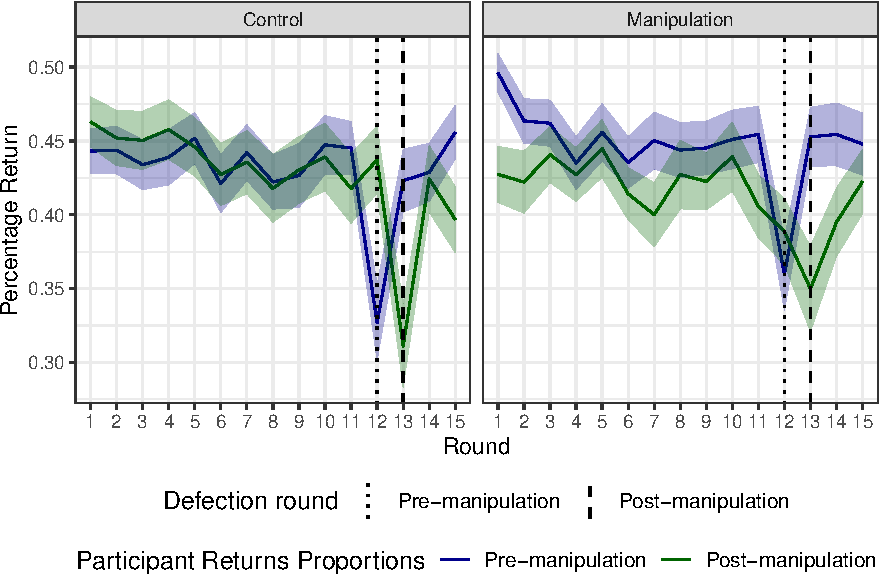
\includegraphics[width=\textwidth]{article_files/figure-latex/gamesPlot-1} 

}

\caption{Averages and standard errors of the trustee's return as a percentage of the multiplied investment received (y-axis) by Condition, Phase, and game round (x-axis) averaged across RS groups. The blue line shows the returns in the Pre phase and the green line those in the Post phase. The left Panel shows returns in the Control condition and the right one those in the Manipulation condition. The dotted lines identify the rounds where the pre-programmed one-off low investment occurs. We note lower average returns post vs pre in the Manipulation condition, whilst returns in the Control condition are similar between the two phases.}\label{fig:gamesPlot}
\end{figure}

Mixed-effects analysis on the percentage returns shows a significant main effect of Phase (Pre vs.~Post RTG game), \(F(1, 201.63) = 5.81\), \(p = .017\), with higher percentage returns in the Pre RTG compared to the Post. Importantly, we also find an interaction between Condition and Phase (RTG pre- vs.~post-manipulation), \(F(1, 201.63) = 4.38\), \(p = .038\). As shown in Figure \ref{fig:boxPlots}, post-hoc tests confirm that, contrary to our expectations, there was a decrease in the percentage returned only in the Manipulation condition, pre - post,
\(\Delta M = 0.03\), 95\% CI \([0.01, 0.05]\), \(t(201.50) = 3.15\), \(p = .002\), but no change in the Control condition. We find no interaction between Phase, Condition and RS, suggesting that there was no difference between RS groups for this interaction.

There was also a significant main effect of Investment,
\(F(1, 5955.67) = 325.35\), \(p < .001\),
such that higher investments were associated with higher percentage returns indicating positive reciprocity. An Investment by Condition interaction,
\(F(1, 5955.67) = 13.92\), \(p < .001\), reflected that returns were more affected by investments in the Control condition. We also find a three way interaction between Phase, Investment and RS, \(F(1, 5864.62) = 7.84\), \(p = .005\), showing that the differentiated effect of the investment on the proportion returned by RS group is itself moderated by the Phase (pre- vs post manipulation). Finally, we find a four-way interaction between Condition, Phase, Investment and RS \(F(1, 5864.62) = 9.24\), \(p = .002\). For completeness, these effects are discussed in more detail in the supplement.

\begin{figure}

{\centering 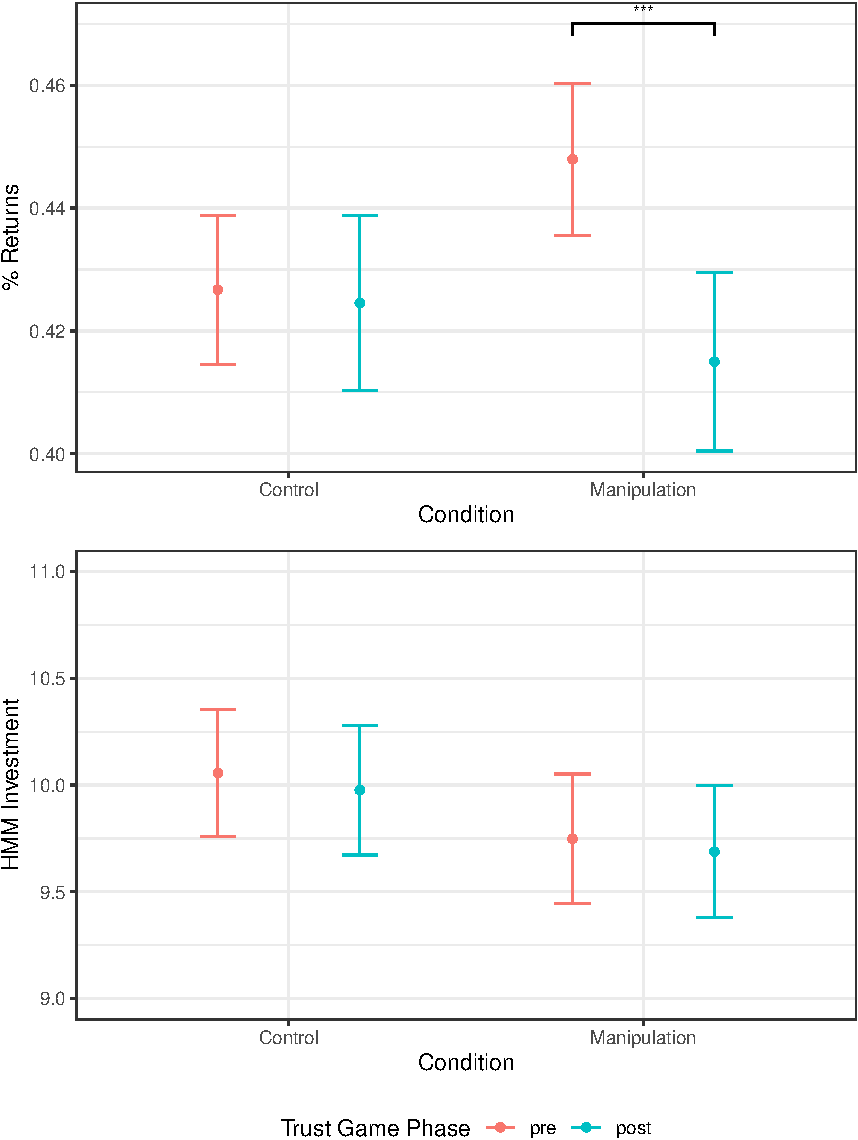
\includegraphics[width=\textwidth]{article_files/figure-latex/boxPlots-1} 

}

\caption{Marginal means and distributions of either investments or percentage returns across participants by Phase and Condition. The top panel shows that participants in the Intervention condition returned lower proportions of the multiplied investment received in the second game compared to the first game over all ronds, whilst those in the Control condition sent back similar returns. The bottom panel shows no difference on aggregate of how the HMM invested across Phases and Conditions.}\label{fig:boxPlots}
\end{figure}

\subsubsection{Post Defection Trials}\label{post-defection-trials}

Did participants learn to be more forgiving and cooperative after witnessing the pre-programmed defection by the HMM investor? To explore this question, we restrict the analysis to the trials following the pre-programmed defection by the HMM agent in both the ``pre'' (trials 12 to 15) and the ``post'' phases (trials 13 to 15). We fit the same mixed effects model as for all the trials with the exception of the RS variable. This is because RS did not show main or interaction effects in the main model, and also due to the necessity of running a simpler model to accommodate the low number of trials. We find a significant main effect of Phase \(F(1, 227.47) = 4.76\), \(p = .030\) with returns lower in the second game post defection trials compared to the first. We also find a main effect of Investment
\(F(1, 1296.14) = 156.41\), \(p < .001\)
where participants continued to return higher proportions when receiving higher investments.
Finally, we still find an Investment by Condition interaction
\(F(1, 5955.67) = 13.92\), \(p < .001\) showing a lower effects of investment on the Manipulation condition compared to the Control condition in post-defection trials. However, the absence of a Condition by Phase effect indicates there was no difference between conditions on participants' reaction to a one-off defection by the co-player.

\subsubsection{HMM Investor in Pre and Post Phases}\label{hmm-investor-in-pre-and-post-phases}

Was the HMM's strategy similar between pre and post phases in the control condition? Was participants' behavior post exposure differentiated enough to induce a different reaction from the HMM? To answer these questions, we test for differences in the HMM agent's investment by Phase, Condition and RS using a linear mixed-effects model as described in the methods section. As seen in Figure \ref{fig:boxPlots}, we find no main or interaction effects, indicating the HMM's behavior was on aggregate similar across levels of Phase, Condition and RS. This consistency in the investor's behavior is a desirable feature of the HMM agent when the participants behavior is largely simialr between phases. More importantly, it indicates that the lower returns of participants in the post phase of the manipulation condition were not differentiated enough to make the HMM react by transitioning to lower latent trust states. It is also noteworthy that the HMM agent was relatively successful in imitating human behavior in this paradigm: When asked during debrief whether they thought the investors they faced were human or not, \(41\)\% of participants thought they were either facing a human or were not sure of the nature of the co-player. When asked to justify their choice, many answers reflected participants projecting human traits such as ``spitefulness'' or ``greed'' onto the artificial co-player's behavior.

\subsubsection{Exposure Phase Trials}\label{exposure-phase-trials}

So far we focused on analysing behavior for the pre and post phases. Here, we look at returns and investments in the exposure phase. The linear mixed effects model of participants' returns in the exposure phase does not show a main effect of Condition on returns. There was a main effect of Investment, \(F(1, 4117.20) = 233.19\), \(p < .001\), with participants positively reciprocating higher investments, an interaction effect between Condition and Investment \(F(1, 4117.20) = 45.93\), \(p < .001\), showing a stronger positive reciprocity in the Control condition, and finally a three way interaction between the RS group, Condition and Investment \(F(1, 4117.20) = 4.21\), \(p = .040\), showing that this stronger positive reciprocity to investment in the Control condition is higher for participants with high RS. The linear mixed effects model of the HMM investments shows a main effect of Condition \(F(1, 202) = 197.64\), \(p < .001\), suggesting higher overall investments for the forgiving HMM compared to the human-like HMM, but no difference in investments when facing low and high RS groups.

In summary, despite the forgiving HMM sending overall higher investments in the exposure phase, participants returned similar proportions of the multiplied investments as those facing the human-like HMM. The positive reciprocity of returns to investments was higher in the Control condition with this relationship stronger for the high RS group.

\subsubsection{Questionnaire Scores and Performance}\label{questionnaire-scores-and-performance}

Whilst we found a significant correlation between participant's Levels of Personality Functioning Score (LPFS) and the Rejection Sensitivity Questionnaire score (RSQ), Spearman's \(r_{\mathrm{s}} = .52\), \(p < 0.001\), there was no correlation between these questionnaire scores and participant's return or overall task performance.

\subsection{Player Ratings}\label{player-ratings}

Figure \ref{fig:plotRatings} shows participants' ratings of each player they faced by condition and RS group. We will focus on two contrasts to analyse the ratings by Condition and RS group. The first is between the rating in the first phase (``pre'') when participants phase the human-like HMM, and the average rating during the exposure phase (average of ``expo1'', ``expo2'' and ``expo3'') where they either face the forgiving HMM (Manipulation condition) or the human-like HMM again (Control condition). The second contrast is between the ``pre'' and ``post'' phases of the experiment where in both conditions participants face the same human-like HMM.

\subsubsection{Comparing Pre and Exposure Ratings}\label{comparing-pre-and-exposure-ratings}

For those with high RS, participants in the Manipulation condition rated the investors they faced in the exposure phase (the forgiving HMM) as more Cooperative \(\Delta M = 2.57\), 95\% CI \([0.84, 4.30]\), \(t(808) = 2.91\), \(p = .004\). There was no difference in ratings on forgiveness and whether they would like to face the co-players again.
Those in the Control condition rated the investors faced in the exposure group (same HMM) as less cooperative \(\Delta M = -2.65\), 95\% CI \([-4.37, -0.94]\), \(t(808) = -3.04\), \(p = .002\), less forgiving \(\Delta M = -2.19\), 95\% CI \([-4.00, -0.39]\), \(t(808) = -2.38\), \(p = .017\), and were less keen on facing them again \(\Delta M = -3.62\), 95\% CI \([-5.73, -1.50]\), \(t(808) = -3.36\), \(p < .001\).

For those with low RS, there was no difference in any of the ratings between the ``pre'' and ``exposure'' phases for the Manipulation condition. For the Control condition, participants indicated less willingness to face the exposure co-player compared to the ``pre'' player, \(\Delta M = -2.43\), 95\% CI \([-4.52, -0.34]\), \(t(808) = -2.29\), \(p = .023\) but also did not differ on cooperation and forgiveness ratings. In summary, those with low RS had a mostly undifferentiated perception of players between the pre and exposure phases, even when the co-player was in fact designed to be more forgiving. In contrast, we see that exposing participants with high RS to a more cooperative and more forgiving agent has compensated for the decrease in ratings that would have occurred if faced with a co-player with the exact same strategy.

\begin{figure}[H]

{\centering 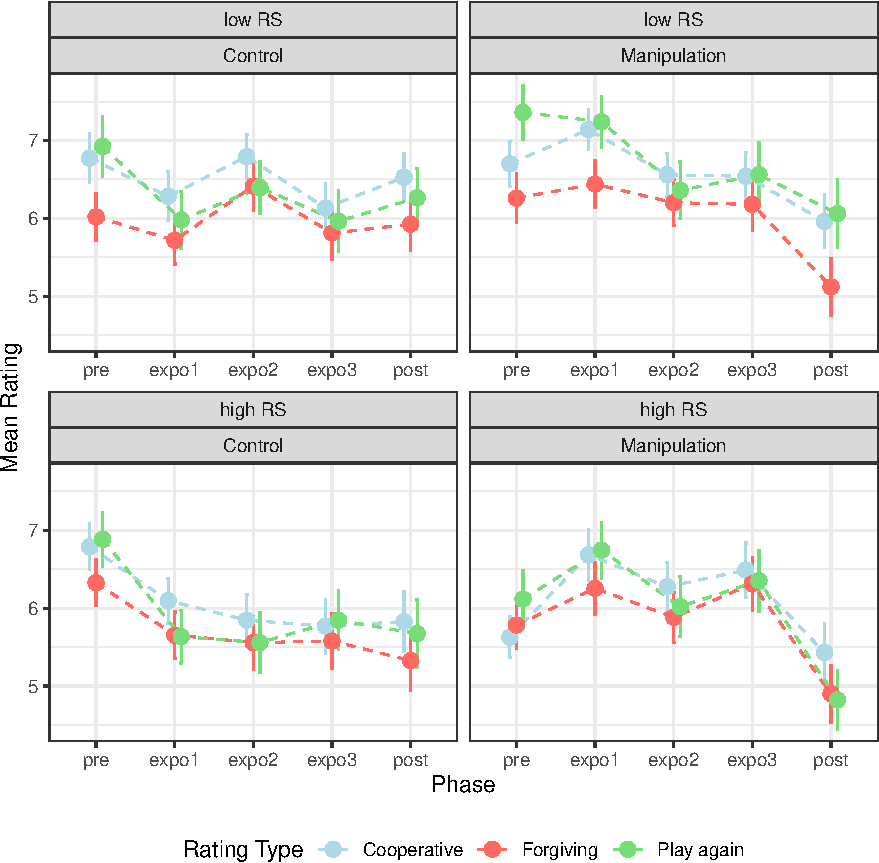
\includegraphics[width=\textwidth]{article_files/figure-latex/plotRatings-1} 

}

\caption{Averages and standard errors of the participants ratings of the opponent (y-axis) by each game and condition for each phase (x-axis). Pre and post are the 15 round RTGs before and after the exposure phase respectively. The games titled expo 1 to 3 are the three 7 round games during the exposure phase. The blue line represents participants' perception of co-player cooperation, the red line indicates perceived co-player forgiveness, and the green line shows the participants' willingness to play again with the same co-player. Cooperation, forgiveness, and willingness to play again ratings remained relatively stable for the low RS group except post-manipulation, where they were lower. In the high RS group, the ratings more accurately reflected the agent's actual cooperativeness and forgiveness in the Manipulation condition, but decreased over time in the Control group. Ratings were also markedly lower in the post-manipulation game for this group.}\label{fig:plotRatings}
\end{figure}

\subsubsection{Comparing Pre and Post Ratings}\label{comparing-pre-and-post-ratings}

Participants high on RS in the Manipulation condition rated the co-players in the ``post'' phase similarly on cooperation, lower on
forgiveness \(\Delta M = -0.88\), 95\% CI \([-1.63, -0.14]\), \(t(808) = -2.33\), \(p = .020\),
and lower on willingness to face them again \(\Delta M = -1.29\), 95\% CI \([-2.16, -0.42]\), \(t(808) = -2.92\), \(p = .004\).
Those in the Control condition rated the investors post the exposure phase lower on all three attributes
(Cooperation: \(\Delta M = -0.96\), 95\% CI \([-1.66, -0.26]\), \(t(808) = -2.70\), \(p = .007\),
Forgiveness: \(\Delta M = -1.00\), 95\% CI \([-1.74, -0.26]\), \(t(808) = -2.66\), \(p = .008\),
Play again: \(\Delta M = -1.21\), 95\% CI \([-2.07, -0.35]\), \(t(808) = -2.76\), \(p = .006\)).

For participants low on RS, those in the Manipulation condition rated the co-players in the ``post'' phase lower on all three attributes
(Cooperation:\(\Delta M = -0.74\), 95\% CI \([-1.45, -0.03]\), \(t(808) = -2.03\), \(p = .042\),
Forgiveness: \(\Delta M = -1.14\), 95\% CI \([-1.89, -0.39]\), \(t(808) = -2.98\), \(p = .003\),
Play again: \(\Delta M = -1.30\), 95\% CI \([-2.18, -0.42]\), \(t(808) = -2.90\), \(p = .004\)).
Those in the Control condition did not differ in their ratings of the ``pre'' and ``post'' phase players.

In summary, we again see that those with low RS accurately perceive the co-player as similar on all attributes throughout the phases in the Control condition. In contrast, the high RS group shows a negative bias towards the co-players after the ``pre'' phase in the Control condition even though the player continues to use the same strategy. After exposure to the forgiving HMM, both groups rate the ``post'' co-player worse than the ``pre'' even though they are the same.

\section{Discussion}\label{discussion}

We used a randomized controlled online experiment where participants played a RTG with artificial agents designed to simulate human-like trust-building scenarios. Participants were then exposed to either forgiving or human-like HMM agents before playing another RTG. Contrary to our hypothesis, exposure to forgiving agents did not increase trust or cooperation. Instead, participants reduced their returns overall whilst the returns of those in the Control group did not change between the pre and post phase of the experiment. Neither did participants show more forgiving behavior in the Manipulation condition after the one-off defection by the agent. Why did participants reduce their returns even though they were repeatedly exposed to more cooperative and more forgiving artificial agents? A look at how the participants rated their co-players might shed some light on what might be driving this reduction in returns for those in the Manipulation condition.

Those exposed to the forgiving agent rated their opponent in the post-exposure phase lower on all attributes even though they faced the same dynamic human-like HMM as pre-exposure. One possible explanation for this drop in rating is that participants exhibited a negative contrast effect. This occurs when the evaluation of a person, object, or situation is influenced by comparisons with recently encountered contrasting objects or people. If we've recently interacted with someone exceptionally nice, our perception of a normal level of niceness might be skewed, making normal behavior seem less favourable or even negative by comparison (Kobre and Lipsitt 1972). As the most recently faced opponents were more forgiving and cooperative, this negative contrast effect may have trumped any learning transfer from being repeatedly exposed to cooperative and forgiving agents (Zentall 2005). If this contrast effect is indeed replicable, then an avenue for future research would be to use it to our benefit by making the participants play agents with low cooperation perception.

It is worth highlighting that RS was not correlated to overall performance in the task. Neither did it moderate the change in returns between Conditions or have an effect on participant returns. However, in examining the player ratings by RS group more closely, we observe that individuals with high RS demonstrate a heightened attunement to changes in the behavior of their HMM co-players: They accurately perceived increased cooperativeness in the forgiving agent, showing an ability to adjust their judgments based on interaction patterns. This may indicate that perceived support from cooperative partners can mitigate their rejection concerns. However, their declining ratings of similar co-players over time, despite consistent agent behavior, suggests that occasional pre-programmed defections may have amplified their perceptions of untrustworthiness and reluctance for future interactions. These nuanced perceptions align with the heightened social awareness often associated with high rejection sensitivity (Downey and Feldman 1996). Individuals with low RS were less affected by the agent's behavioral variations, showing a less volatile baseline of social perception. They still exhibit behavior consistent with a contrast effect in the Manipulation condition. This stability in perception might reflect a lower propensity to scrutinize social cues or a more robust internal model of social interactions that is less easily perturbed by short-term variations in partner behavior.

Despite these differences in perception, the actual cooperative behavior -- as measured by returns in the trust game -- did not significantly differ between RS groups. This suggests a potential dissociation between the cognitive-perceptual processes involved in evaluating social partners and the behavioral output in economic games. There are multiple potential explanations for this: First, the ratings may reflect explicit, conscious evaluations of social partners, while behavior in the trust game might be guided more by implicit, automatic processes that are less differentiated between RS groups. This interpretation aligns with dual-process theories of social cognition (Lieberman 2007). Second, the structured nature of the trust game might provide a context where the behavioral expression of rejection sensitivity is attenuated. In contrast, the more open-ended nature of providing ratings might allow for greater expression of RS-related perceptual biases.

These findings suggest that interventions focused solely on altering behavior might be insufficient, as the underlying perceptual and cognitive processes may remain unchanged. Conversely, therapies targeting these perceptual processes might not necessarily translate into immediate behavioral changes. Future research should investigate whether this dissociation between perception and behavior persists in more naturalistic social interactions or over longer periods. Additionally, exploring specific conditions or thresholds under which perceptual differences begin to manifest in behavioral divergences could provide valuable insights into the dynamics of rejection sensitivity. Simply exposing individuals to highly cooperative or forgiving partners may not suffice to induce lasting changes in behavior. Instead, interventions may need to incorporate more nuanced approaches that gradually shape expectations and behaviors over time. Combining periods of forgiveness with clear communication about mutual expectations for cooperation might be more effective (Balliet, Mulder, and Van Lange 2011). Future studies should also consider the temporal dynamics of these effects, examining whether longer exposure periods or different patterns of forgiving behavior could lead to more positive outcomes. Moreover, investigating the role of explicit communication and meta-cognitive reflection on the cooperative process could offer insights into leveraging positive interactions to promote enduring cooperative tendencies.

\section{Conclusion}\label{conclusion}

This randomised controlled experiment enabled us to uncover unexpected effects of exposure to forgiving behavior on subsequent cooperation, particularly in relation to rejection sensitivity. These findings challenge existing assumptions about fostering cooperative behavior and suggest the need for more nuanced interventions. Importantly, the use of HMM-based artificial agents in this study represents a significant methodological advancement. By providing a balance between experimental control and realistic, adaptive behavior, these agents allowed for a nuanced exploration of trust dynamics that would be challenging to achieve with human confederates or simplistic computer algorithms. This approach opens up new possibilities for studying complex social interactions in controlled settings, potentially bridging the gap between laboratory experiments and real-world social dynamics.

\pagebreak

\section*{Author contributions statement}\label{author-contributions-statement}
\addcontentsline{toc}{section}{Author contributions statement}

I. Guennouni, G. Koppe and C. Korn. designed and developed the study concept. Experiment design, testing and data collection were performed by I. Guennouni. I. Guennouni analysed and interpreted the data under the supervision of G. Koppe and C. Korn. All authors jointly wrote and approved the final version of the manuscript for submission.

\section*{Funding}\label{funding}
\addcontentsline{toc}{section}{Funding}

This publication was supported through state funds approved by the State Parliament of Baden-Württemberg for the Innovation Campus Health + Life Science alliance Heidelberg Mannheim. I. Guennouni was supported by a research fellowship from the AI Health Innovation Cluster

\section*{Competing interests statement}\label{competing-interests-statement}
\addcontentsline{toc}{section}{Competing interests statement}

The author(s) declared that there were no conflicts of interest with respect to the authorship or the publication of this article.

\section*{Additional information}\label{additional-information}
\addcontentsline{toc}{section}{Additional information}

\subsection*{Correspondence}\label{correspondence}
\addcontentsline{toc}{subsection}{Correspondence}

All correspondence and requests for materials should be addressed to I. Guennouni.

\subsection*{Transparency and data availability}\label{transparency-and-data-availability}
\addcontentsline{toc}{subsection}{Transparency and data availability}

Preregistration: The hypotheses and methods were not preregistered.The analysis plan was not preregistered. Materials: All study materials are publicly available (\url{https://github.com/ismailg/exposure-public}). Data: All primary data are publicly available (\url{https://github.com/ismailg/exposure-public}). Analysis scripts: All analysis scripts are publicly available (\url{https://github.com/ismailg/exposure-public}).

\section*{References}\label{references}
\addcontentsline{toc}{section}{References}

\phantomsection\label{refs}
\begin{CSLReferences}{1}{0}
\bibitem[\citeproctext]{ref-abramov_influence_2022-1}
Abramov, Gamze, Jason Kautz, Sebastien Miellet, and Frank P. Deane. 2022. {``The {Influence} of {Attachment Style}, {Self-protective Beliefs}, and {Feelings} of {Rejection} on the {Decline} and {Growth} of {Trust} as a {Function} of {Borderline Personality Disorder Trait Count}.''} \emph{Journal of Psychopathology and Behavioral Assessment} 44 (3): 773--86. \url{https://doi.org/10.1007/s10862-022-09965-9}.

\bibitem[\citeproctext]{ref-almaatouq_empirica_2021}
Almaatouq, Abdullah, Joshua Becker, James P. Houghton, Nicolas Paton, Duncan J. Watts, and Mark E. Whiting. 2021. {``Empirica: A Virtual Lab for High-Throughput Macro-Level Experiments.''} \emph{Behavior Research Methods} 53 (5): 2158--71. \url{https://doi.org/10.3758/s13428-020-01535-9}.

\bibitem[\citeproctext]{ref-american_psychiatric_association_diagnostic_2013}
American Psychiatric Association. 2013. \emph{Diagnostic and {Statistical Manual} of {Mental Disorders}}. Fifth Edition. American Psychiatric Association. \url{https://doi.org/10.1176/appi.books.9780890425596}.

\bibitem[\citeproctext]{ref-balliet_reward_2011}
Balliet, Daniel, Laetitia B. Mulder, and Paul A. M. Van Lange. 2011. {``Reward, Punishment, and Cooperation: {A} Meta-Analysis.''} \emph{Psychological Bulletin} 137 (4): 594--615. \url{https://doi.org/10.1037/a0023489}.

\bibitem[\citeproctext]{ref-bandura_social_1977}
Bandura, Albert. 1977. \emph{Social {Learning Theory}}. Prentice Hall.

\bibitem[\citeproctext]{ref-bowlby_attachment_1978}
Bowlby, John. 1978. {``Attachment Theory and Its Therapeutic Implications.''} \emph{Adolescent Psychiatry} 6: 5--33.

\bibitem[\citeproctext]{ref-charness_investment_2008}
Charness, Gary, Ramón Cobo-Reyes, and Natalia Jiménez. 2008. {``An Investment Game with Third-Party Intervention.''} \emph{Journal of Economic Behavior \& Organization} 68 (1): 18--28. \url{https://doi.org/10.1016/j.jebo.2008.02.006}.

\bibitem[\citeproctext]{ref-downey_implications_1996}
Downey, Geraldine, and Scott I. Feldman. 1996. {``Implications of Rejection Sensitivity for Intimate Relationships.''} \emph{Journal of Personality and Social Psychology} 70 (6): 1327--43. \url{https://doi.org/10.1037/0022-3514.70.6.1327}.

\bibitem[\citeproctext]{ref-downey_early_1997}
Downey, Geraldine, Hala Khouri, and Scott I. Feldman. 1997. {``Early Interpersonal Trauma and Later Adjustment: {The} Mediational Role of Rejection Sensitivity.''} In \emph{Developmental Perspectives on Trauma: {Theory}, Research, and Intervention}, 85--114. Rochester Symposium on Developmental Psychology, {Vol}. 8. Rochester, NY, US: University of Rochester Press.

\bibitem[\citeproctext]{ref-fiedler_social_2011}
Fiedler, Marina, Ernan Haruvy, and Sherry Xin Li. 2011. {``Social Distance in a Virtual World Experiment.''} \emph{Games and Economic Behavior} 72 (2): 400--426. \url{https://doi.org/10.1016/j.geb.2010.09.004}.

\bibitem[\citeproctext]{ref-fonagy_mentalizing_2017}
Fonagy, Peter, and Chloe Campbell. 2017. {``\href{https://www.ncbi.nlm.nih.gov/pubmed/29135441}{Mentalizing, Attachment and Epistemic Trust: How Psychotherapy Can Promote Resilience}.''} \emph{Psychiatria Hungarica: A Magyar Pszichiatriai Tarsasag Tudomanyos Folyoirata} 32 (3): 283--87.

\bibitem[\citeproctext]{ref-fowler_cooperative_2010}
Fowler, James H., and Nicholas A. Christakis. 2010. {``Cooperative Behavior Cascades in Human Social Networks.''} \emph{Proceedings of the National Academy of Sciences} 107 (12): 5334--38. \url{https://doi.org/10.1073/pnas.0913149107}.

\bibitem[\citeproctext]{ref-gao_associations_2017}
Gao, Shuling, Mark Assink, Andrea Cipriani, and Kangguang Lin. 2017. {``Associations Between Rejection Sensitivity and Mental Health Outcomes: {A} Meta-Analytic Review.''} \emph{Clinical Psychology Review} 57 (November): 59--74. \url{https://doi.org/10.1016/j.cpr.2017.08.007}.

\bibitem[\citeproctext]{ref-hepp_prosociality_2022}
Hepp, Johanna, and Inga Niedtfeld. 2022. {``Prosociality in Personality Disorders: {Status} Quo and Research Agenda.''} \emph{Current Opinion in Psychology} 44 (April): 208--14. \url{https://doi.org/10.1016/j.copsyc.2021.09.013}.

\bibitem[\citeproctext]{ref-herpertz_social-cognitive_2014}
Herpertz, Sabine C., and Katja Bertsch. 2014. {``The Social-Cognitive Basis of Personality Disorders.''} \emph{Current Opinion in Psychiatry} 27 (1): 73--77. \url{https://doi.org/10.1097/YCO.0000000000000026}.

\bibitem[\citeproctext]{ref-joyce_trust_1995}
Joyce, Berg, John Dickhaut, and Kevin McCabe. 1995. {``Trust, {Reciprocity}, and {Social History}.''} \emph{Games and Economic Behavior} 10 (1): 122--42.

\bibitem[\citeproctext]{ref-king-casas_getting_2005}
King-Casas, Brooks, Damon Tomlin, Cedric Anen, Colin F. Camerer, Steven R. Quartz, and P. Read Montague. 2005. {``Getting to {Know You}: {Reputation} and {Trust} in a {Two-Person Economic Exchange}.''} \emph{Science} 308 (5718): 78--83. \url{https://doi.org/10.1126/science.1108062}.

\bibitem[\citeproctext]{ref-kobre_negative_1972}
Kobre, Kenneth R, and Lewis P Lipsitt. 1972. {``A Negative Contrast Effect in Newborns.''} \emph{Journal of Experimental Child Psychology} 14 (1): 81--91. \url{https://doi.org/10.1016/0022-0965(72)90033-1}.

\bibitem[\citeproctext]{ref-lieberman_social_2007}
Lieberman, Matthew D. 2007. {``Social {Cognitive Neuroscience}: {A Review} of {Core Processes}.''} \emph{Annual Review of Psychology} 58 (1): 259--89. \url{https://doi.org/10.1146/annurev.psych.58.110405.085654}.

\bibitem[\citeproctext]{ref-matuschek_balancing_2017}
Matuschek, Hannes, Reinhold Kliegl, Shravan Vasishth, Harald Baayen, and Douglas Bates. 2017. {``Balancing {Type I} Error and Power in Linear Mixed Models.''} \emph{Journal of Memory and Language} 94 (June): 305--15. \url{https://doi.org/10.1016/j.jml.2017.01.001}.

\bibitem[\citeproctext]{ref-miano_rejection_2013}
Miano, Annemarie, Eric A. Fertuck, Arnoud Arntz, and Barbara Stanley. 2013. {``Rejection {Sensitivity Is} a {Mediator Between Borderline Personality Disorder Features} and {Facial Trust Appraisal}.''} \emph{Journal of Personality Disorders} 27 (4): 442--56. \url{https://doi.org/10.1521/pedi_2013_27_096}.

\bibitem[\citeproctext]{ref-mikulincer_attachment_1998}
Mikulincer, Mario. 1998. {``Attachment Working Models and the Sense of Trust: {An} Exploration of Interaction Goals and Affect Regulation.''} \emph{Journal of Personality and Social Psychology} 74 (5): 1209--24. \url{https://doi.org/10.1037/0022-3514.74.5.1209}.

\bibitem[\citeproctext]{ref-mulder_relationship_1999}
Mulder, R. T., P. R. Joyce, P. F. Sullivan, C. M. Bulik, and F. A. Carter. 1999. {``The Relationship Among Three Models of Personality Psychopathology: {DSM-III-R} Personality Disorder, {TCI} Scores and {DSQ} Defences.''} \emph{Psychological Medicine} 29 (4): 943--51. \url{https://doi.org/10.1017/S0033291799008533}.

\bibitem[\citeproctext]{ref-richetin_emotional_2018}
Richetin, Juliette, Anita Poggi, Paola Ricciardelli, Eric A. Fertuck, and Emanuele Preti. 2018. {``The Emotional Components of Rejection Sensitivity as a Mediator Between {Borderline Personality Disorder} and Biased Appraisal of Trust in Faces.''} \emph{Clinical Neuropsychiatry: Journal of Treatment Evaluation} 15 (4): 200--205.

\bibitem[\citeproctext]{ref-singmann_afex_2022}
Singmann, Henrik, Ben Bolker, Jake Westfall, Frederik Aust, Mattan S. Ben-Shachar, Søren Højsgaard, John Fox, et al. 2022. {``Afex: {Analysis} of {Factorial Experiments}.''}

\bibitem[\citeproctext]{ref-weekers_level_2019}
Weekers, Laura C., Joost Hutsebaut, and Jan H. Kamphuis. 2019. {``The {Level} of {Personality Functioning Scale}-{Brief Form} 2.0: {Update} of a Brief Instrument for Assessing Level of Personality Functioning.''} \emph{Personality and Mental Health} 13 (1): 3--14. \url{https://doi.org/10.1002/pmh.1434}.

\bibitem[\citeproctext]{ref-zentall_within-trial_2005}
Zentall, Thomas R. 2005. {``A {Within-trial Contrast Effect} and Its {Implications} for {Several Social Psychological Phenomena}.''} \emph{International Journal of Comparative Psychology} 18 (4). \url{https://doi.org/10.46867/ijcp.2005.18.04.08}.

\end{CSLReferences}

\end{document}
